The CDCL solver creates and handles a particular data structure, called \textbf{implication graph}, mainly used to save several information. They will be used 
to perform \textbf{Backjumping} activities when necessary. \vspace{7pt}

An implication graph ($G = (V, E)$) is a directed acyclic graph that records the history of decisions and the resulting deductions derived during the unit
propagation processes:
\begin{itemize}
    \renewcommand{\labelitemi}{-}
    \item Each node $v$, with $v \in V$, represents a decision, a derived literal or a conflict. We label any node by a certain decision level $d$, so for instance the node $k@d$ describes a contradiction reached at a specific level $d$ of the graph.
    \item Every edge $v \xrightarrow{c_i} w \in E$ indicates that $w$ is derived with unit propagation from the clause $c_i$ with one of its literals being $v$ (\textit{therefore, $v$ and $w$ share at least one clause}).
\end{itemize}
\begin{example}
    e.g. Implication graph. \vspace{7pt}

    Starting from the following list of clauses:
    \begin{enumerate}
        \item $\neg x_1 \vee x_2 \vee \neg x_4$
        \item $\neg x_1 \vee \neg x_2 \vee x_3$ 
        \item $\neg x_3 \vee \neg x_4$ 
        \item $x_4 \vee x_5 \vee x_6$ 
        \item $\neg x_5 \vee x_7$ 
        \item $\neg x_6 \vee x_7 \vee \neg x_8$ 
    \end{enumerate}
    Define if the whole CNF propositional formula is satisfiable or unsatisfiable. \vspace{7pt}

    \textbf{Resolution}. \\
    We start randomly taking in account the boolean variable $x_1$, assigning a true value to it. Then, we create a node in our implication graph 
    with a decision level $d$ equal to $1$, since it's the first level of the data structure. \vspace{3.5pt}
    \begin{center}
        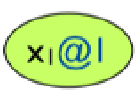
\includegraphics[width = 0.15\textwidth]{img/img31.png}
    \end{center} \vspace{3.5pt}
    We move to the second level, choosing the variable $x_8$, taking also for it a true value. \vspace{3.5pt}
    \begin{center}
        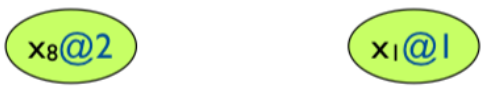
\includegraphics[width = 0.5\textwidth]{img/img32.png}
    \end{center} \vspace{3.5pt}
    Now, we take in consideration at the third level the variable $x_7$, putting it to false. However, we can derive by unit propagation the term $\neg x_5$ from 
    the fifth clause. This will be out first edge ever. \vspace{3.5pt}
    \begin{center}
        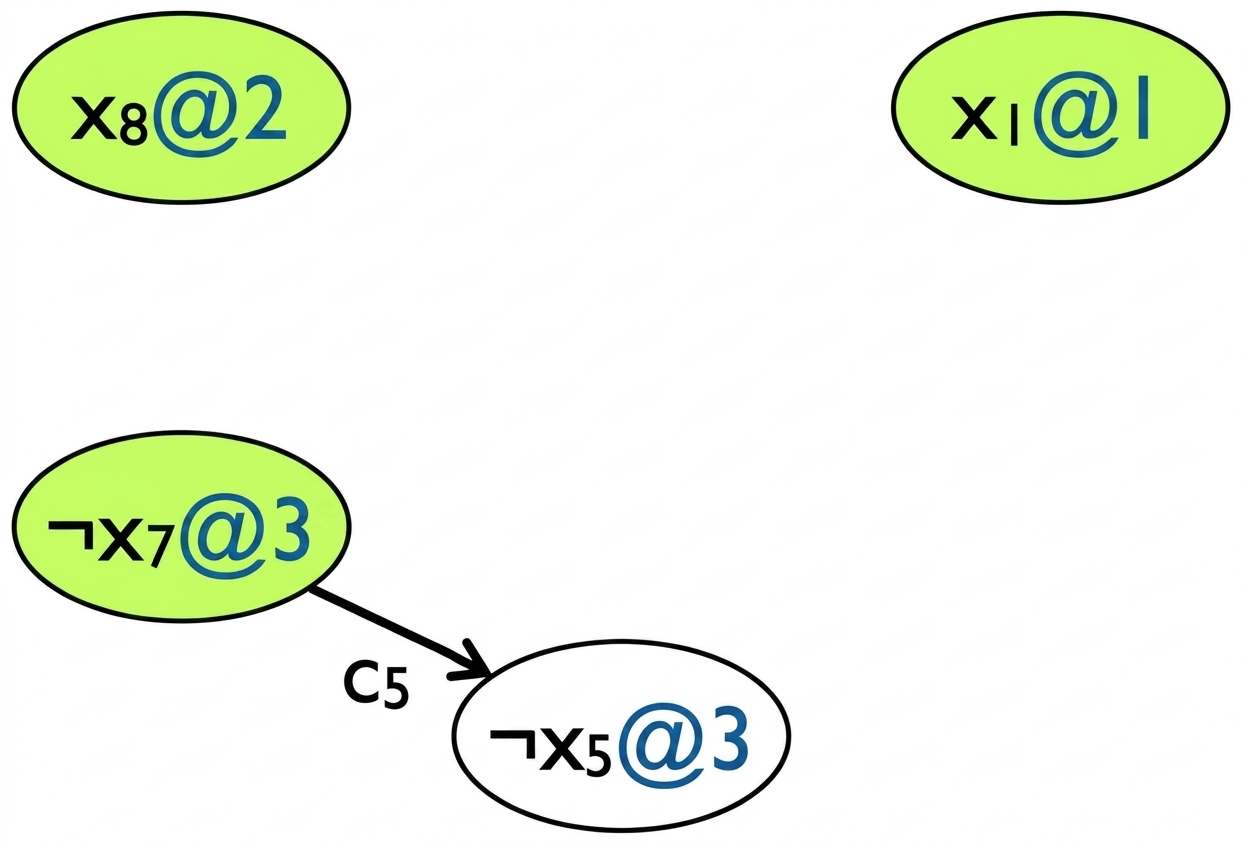
\includegraphics[width = 0.5\textwidth]{img/img33.png}
    \end{center} \vspace{3.5pt}
    As we can observe from the image above, we have built a new node for $x_5$ boolean variable, maintaining the same decision level. $\neg x_5$ and $x_7$ are 
    linked by an edge labelled by the clause that combines them together. \vspace{7pt}

    After we introduced $x_7$ node, we can also add $\neg x_6$ in the graph, derived from the sixth clause. The node $\neg x_6$ has the same decision level of 
    $x_7$ and $x_8$, and it takes false as value. \vspace{3.5pt}

    Additionally, from the fourth clause we could derive $x_4$: it must be true in order to satisfy the propositional formula. \vspace{3.5pt}
    \begin{center}
        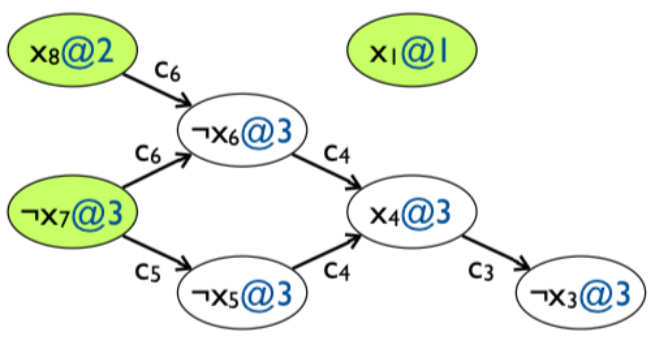
\includegraphics[width = 0.5\textwidth]{img/img34.png}
    \end{center} \vspace{3.5pt}
    We keep going until we reach a contradiction or the satisfiability of the problem. However, taking these truth values we reach a contradiction: in the second
    clause ($\neg x_1 \vee \neg x_2 \vee x_3$) both $x_1$ and $x_2$ are set to true and $x_3$ is set to false, reaching a conflict between them. Therefore, in the 
    implication graph, we would create a node also for the conflict. \vspace{3.5pt}
    \begin{center}
        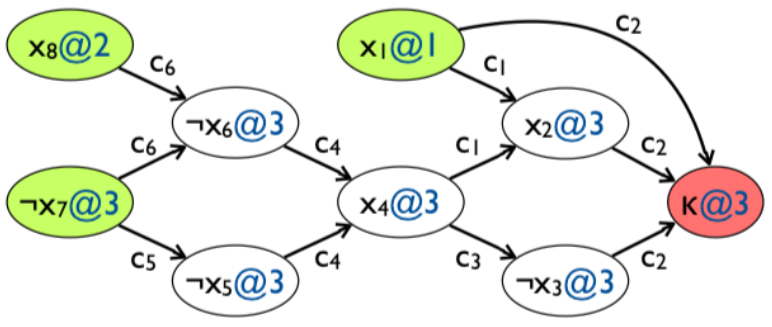
\includegraphics[width = 0.6\textwidth]{img/img35.png}
    \end{center} \vspace{3.5pt}
    How can we derive new truth values from this graph? First of all, we apply the unit resolution between the first and second clauses. But, also the third clause
    is involved in the contradiction, so it's another entity to take in account in the resolution process. Anyway, at the same time we can state that $\neg x_4$
    comes from the fourth clause and it has a direct influence on $x_2$ and $x_3$; so, maybe, also the fourth clause might be considered in the unit resolution 
    mechanism. This type of reasoning keeps going until we cover the whole list of clauses, formally it can be expressed as follows:
    \begin{itemize}
        \renewcommand{\labelitemi}{-}
        \item $\neg x_1 \vee x_3 \vee \neg x_4$ ($c_1$ and $c_2$)
        \item $\neg x_1 \vee \neg x_4$ ($c_*$ and $c_3$)
        \item $\neg x_1 \vee x_5 \vee x_6$ ($c_*$ and $c_4$)
        \item $\neg x_1 \vee x_6 \vee x_7$ ($c_*$ and $c_5$)
        \item $\neg x_1 \vee x_7 \vee \neg x_8$ ($c_*$ and $c_6$)
    \end{itemize} \vspace{7pt}

    Note: with $c_k$ with $k \in \{1, 2, 3, 4, 5, 6\}$ we mean the clauses of the original list. With $c_*$ we mean the clause derived during the unit propagation. \vspace{7pt}

    Right now, from the unit propagation process we know that only $x_1$ and $x_8$ can be false and $x_7$ must be set to true. However, instead of going 
    back so far until the beginnig, we could stop somewhere in the middle, since we have already found something new. \vspace{7pt}

    We got several back-steps from the previous list, but how can we choose the \textbf{more valid backjump}? In almost of the cases, we consider the definition
    of \textbf{unit implication point}. 
    \begin{definition}
        An unit implication point is any node in the implication graph that is part of all the paths from the current decision literal ($l@d$) to the 
        conflict ($k@d$). \vspace{7pt}

        In particular, the \textbf{first unit implication point} (\textit{1UIP}) is the implication point which is closest to the conflict. 
    \end{definition} 
    Normally, we will backjump at the decision $x_7$, but now we are gonna to come back on $x_1$ and $x_4$, since we learnt that both variables 
    cannot be assigned to the same value. \vspace{7pt}

    Therefore, the first step is to add the new clause ($\neg x_1 \vee \neg x_4$) inside the list of clauses.
    \begin{itemize}
        \renewcommand{\labelitemi}{-}
        \item $\neg x_1 \vee x_3 \vee \neg x_4$ ($c_1$ and $c_2$)
        \item $\neg x_1 \vee \neg x_4$ ($c_*$ and $c_3$)
        \item $\neg x_1 \vee x_5 \vee x_6$ ($c_*$ and $c_4$)
        \item $\neg x_1 \vee x_6 \vee x_7$ ($c_*$ and $c_5$)
        \item $\neg x_1 \vee x_7 \vee \neg x_8$ ($c_*$ and $c_6$)
        \item $\neg x_1 \vee \neg x_4$
    \end{itemize} \vspace{7pt}

    Previously, we reached a contradiction by the following unit propagation:
    $$ x_1^d \ x_8^d \ x_7^d \ \neg x_6 \ \neg x_5 \  x_4 \ x_2 \ \neg x_3 $$
    however, as we discussed before, thanks to $\neg x_1 \vee \neg x_4$ we learnt that there was an unit propagation setting $x_4$ to the wrong truth value.
    Therefore, we can start again from the decisional node $x_1$:
    $$ x_1^d \ \neg x_4$$
\end{example}